\apendice{Plan de Proyecto Software}

\section{Introducción}

En este apéndice se ha recogido la planificación temporal, estudio de viabilidad y viabilidad legal.

\section{Planificación temporal}

Para realizar la planificación temporal se ha utilizado la metodología de gestión ágil de proyectos (Scrum). La planificación del proyecto se realizó desde GitHub junto con la extensión Zenhub. En estas herramientas de gestión de versiones se realizaron varios sprints de trabajo con una duración aproximada de 2 semanas. En estos periodos de tiempo se han definido tareas a completar. 

Estas tareas o \textit{issues} están asignadas a una persona, tienen una etiqueta de cara a su organización y una estimación de la dificultad. En cuanto a las etiquetas o labels, en este proyecto se han trabajado con las predefinidas por GitHub siendo estas:
\begin{itemize}
    \item \textbf{Enhacement:} Añade una nueva característica o petición. Se puede ver con mayor detalle en \href{https://github.com/humbertoms99/Mixing_models/issues?q=label%3Aenhancement+}{Enhacement}.
    \item \textbf{Bug:} Corrección de errores o funcionamientos incorrectos de la aplicación. Se puede ver con mayor detalle en \href{https://github.com/humbertoms99/Mixing_models/issues?q=label%3Abug+}{Bug}.
    \item \textbf{Documentation:} Tareas de documentación, en las que se espera añadir o mejorar documentos. Se puede ver con mayor detalle en \href{https://github.com/humbertoms99/Mixing_models/issues?q=label%3Adocumentation}{Documentation}.  
    \item \textbf{Duplicate:} Referentes a issues ya existentes.
    \item \textbf{Good first issue:} Tareas para facilitar el uso a nuevos usuarios. Se puede ver con mayor detalle en  \href{https://github.com/humbertoms99/Mixing_models/issues?q=label%3A%22good+first+issue%22}{Good first issue}.
    \item \textbf{Help wanted:} Tareas que requieren ayuda externa.
    \item \textbf{Invalid:} Tareas incorrectas.
    \item \textbf{Question:} Se solicita más información.
    \item \textbf{Wontfix:} Tareas que no han sido resueltas o que no están funcionando en ese momento.
\end{itemize}

\subsection{Sprints del proyecto}

Antes de comenzar con el desarrollo de funcionalidades para la aplicación se realizaron algunas tareas previas como: decisión de lenguajes con los que trabajar, herramientas a utilizar y un periodo de formación.

Antes de empezar con cualquier desarrollo se realizó un curso de \LaTeX (Más información en la issue \href{https://github.com/humbertoms99/Mixing_models/issues/1}{Curso de para aprender a usar Latex}) con el objetivo de poder documentar a la vez que se añadían funcionalidades. A continuación, se realizaron algunas tareas de análisis de la herramienta GitHub para comprender en profundidad sus posibilidades. Se leyeron algunos artículos sobre las \href{https://github.com/humbertoms99/Mixing_models/issues/2}{\textit{Milestones} y \textit{Sprints}}, junto con una aproximación a los \href{https://github.com/humbertoms99/Mixing_models/issues/3}{\textit{GitHub Reports}}.

También se preparó el entorno de desarrollo, descargando algunas herramientas como: Instalación Visual Studio Code y configuración extensiones para trabajar con Angular, Postman, extensión de ZenHub, Debian y Mendeley inicialmente.

\subsubsection{Sprints análisis}

Previo al desarrollo de funcionalidades se lleva a cabo una etapa de análisis. Durante estas semanas se realizó un análisis en profundidad del artículo \textit{Using n-alkanes to estimate diet composition of herbivores} \cite{problemn-alkanes2007}. Durante este periodo se aprendió sobre cómo resolver sistemas de ecuaciones con restricciones. Se resolvieron ejercicios en Matlab para entender aun más en profundidad los pasos para resolver estos sistemas. 

Una vez se definió y entendió el problema planteado se realizó una búsqueda de librerías y lenguajes para desarrollar posteriormente la aplicación.  

\subsubsection{Sprints iniciales}

Durante los primeros meses se realizó la instalación de la librería GLPK \cite{glpk:package} y se realizaron algunos ejemplos para llamar desde una proyecto front a una API que realizara funcionalidades de la librería, en concreto resolviera problemas de programación lineal, y recibiéramos esos resultados desde el proyecto front. 

\subsubsection{Sprint: 17 Mayo - 31 Mayo, 2022}

Una vez se conectaron los dos proyectos se empezaron a desarrollar de forma simultánea tanto la API como el front, utilizando la herramienta Postman para hacer pruebas de peticiones.

Este sprint se centró en realizar un flujo en el cual se introducían los datos desde el front y por medio de una petición al API escrita en laravel se recibía la respuesta al problema. A partir de la cual se hizo una primera visual de los resultados.

Las tareas completadas son representadas en el gráfico de la figura \ref{fig:sprint_17_31_may}.

\begin{itemize}
    \item \textbf{\#4-Resolver problemas Non-negative least square, min y max desde api laravel}.
    \item \textbf{\#5-Realizar ciclo de recepción y mostrar los resultados desde la web}.
    \item \textbf{\#6-Subida documentación y códigos}.
\end{itemize}

\begin{figure}[h!] 
\centering
    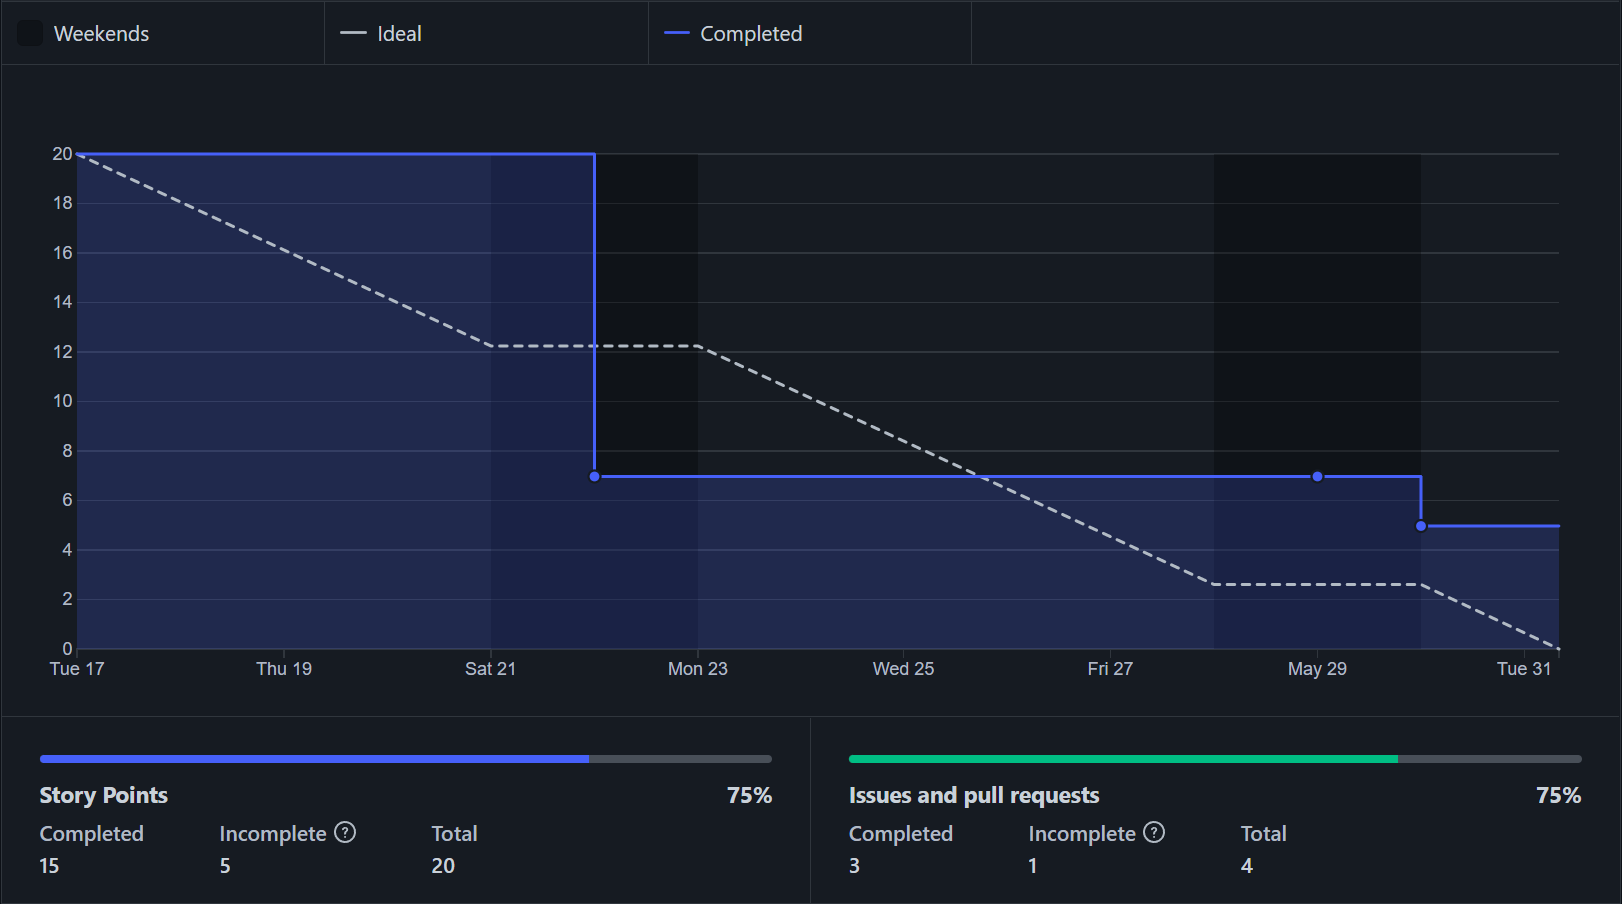
\includegraphics[width=0.8\textwidth]{img/sprint_17_31_may.PNG}
\caption{Sprint: 17 Mayo - 31 Mayo, 2022}
\label{fig:sprint_17_31_may}
\end{figure}

\newpage

\subsubsection{Sprint: 31 Mayo - 14 Junio, 2022}

Este sprint se centró principalmente en preparar los documentos para importar y exportar, preparando también todo el sistema de carga de archivos de la web. Además de configurar los ficheros de traducciones en la web.

\begin{itemize}
    \item \textbf{\#7-Funcionamiento paquete GLPK}.
    \item \textbf{\#8-Alert proyección no coincidente con punto}.
    \item \textbf{\#9-Exports solución y datos problemas}.
    \item \textbf{\#10-Descargar .mod de cada elemento de la solución}.
    \item \textbf{\#11-Import datos problema}.
    \item \textbf{\#12-Sistema de Traducciones}.
    \item \textbf{\#14-Export csv traducidos}.
\end{itemize}

Podemos ver el gráfico correspondiente a las tareas anteriores en la figura \ref{fig:sprint_31_14_jun}.

\begin{figure}[h!] 
\centering
    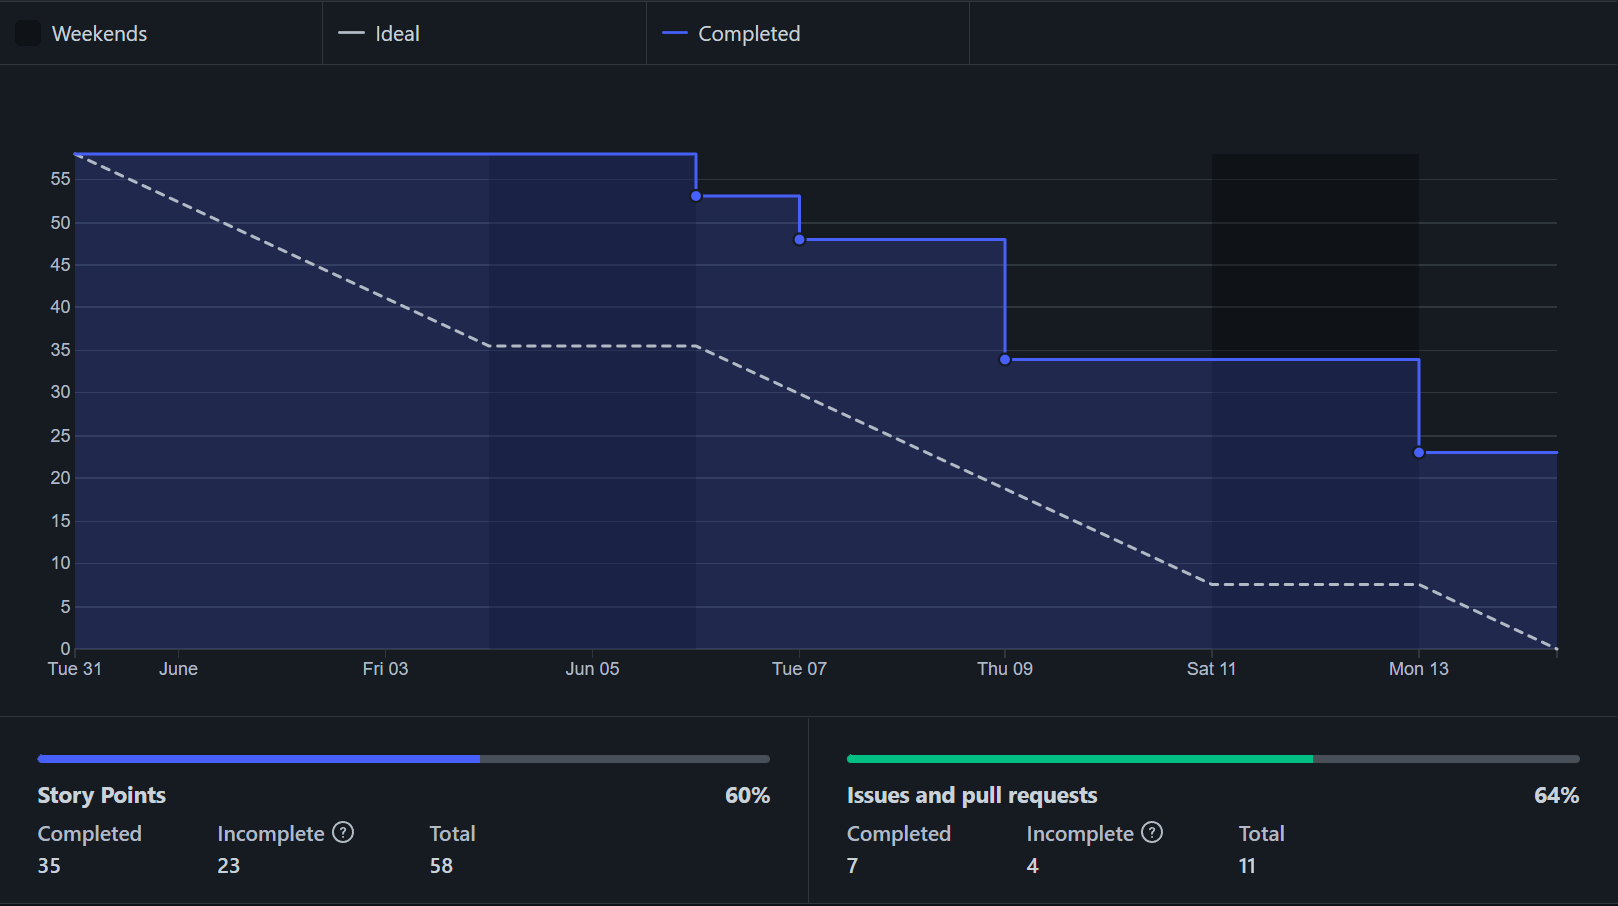
\includegraphics[width=0.8\textwidth]{img/sprint_31_14_jun.PNG}
\caption{Sprint: 31 Mayo - 14 Junio, 2022}
\label{fig:sprint_31_14_jun}
\end{figure}

\subsubsection{Sprint: 14 Junio - 28 Junio, 2022}

Este Sprint está marcado principalmente por la subida a un servidor de nuestro proyecto, aunque también se hicieron pequeños ajustes de maquetación y procedimientos de cara a agilizar el uso de la aplicación

\begin{itemize}
    \item \textbf{\#13-Slider web}.
    \item \textbf{\#15-Ajustes maquetación solución}.
    \item \textbf{\#16-Subida a servidor}.
    \item \textbf{\#17-Función reset arrays}.
    \item \textbf{\#19-Añadir línea min max en exports solución}.
\end{itemize}

Podemos ver el gráfico \textit{"Burndown report"} correspondiente al sprint en la figura \ref{fig:sprint_14_28_jun}.

\begin{figure}[h!] 
\centering
    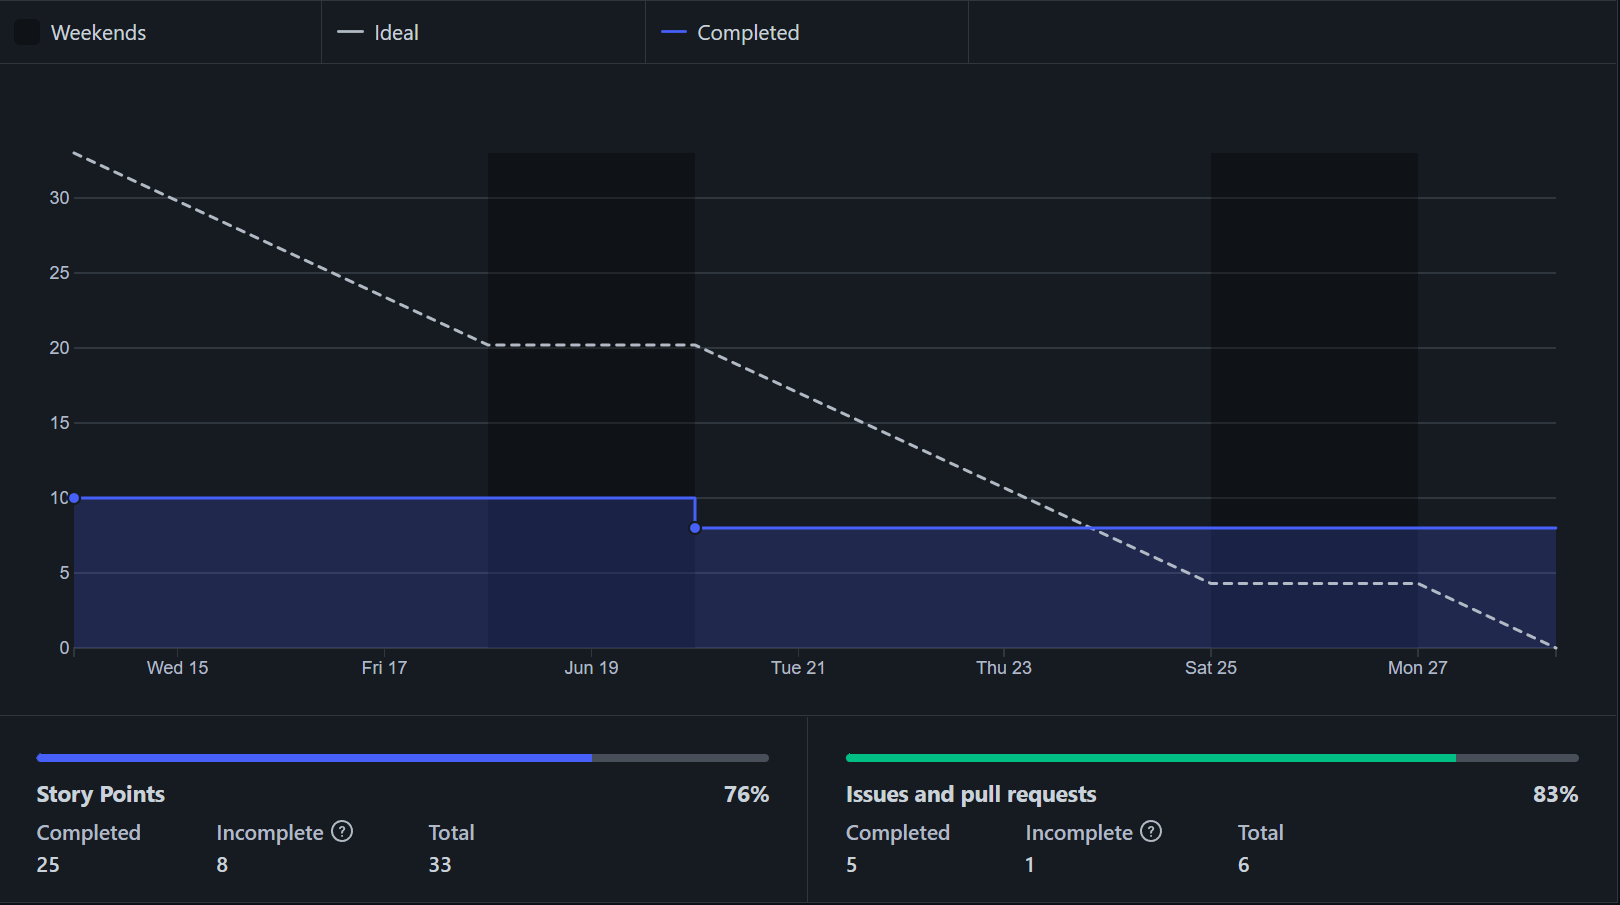
\includegraphics[width=0.8\textwidth]{img/sprint_14_28_jun.PNG}
\caption{Sprint: 14 Mayo - 28 Junio, 2022}
\label{fig:sprint_14_28_jun}
\end{figure}

\newpage
\subsubsection{Sprint: 6 Septiembre - 20 Septiembre, 2022}

En este último sprint se han añadido cambios para adaptar por completo las funciones a la nueva librería, se han resuelto algunos bugs, y se ha realizado la primera versión de los documentos memoria y anexos.

\begin{itemize}
    \item \textbf{\#18-Primera versión memoria}
    \item \textbf{\#23-Búsqueda funciones resuelvan las funciones usadas en el API}
    \item \textbf{\#24-Cambio función api "deleteAllfiles()" al proyecto front}
    \item \textbf{\#25-Cambio función API - "getTextFiles()" al proyecto front}
    \item \textbf{\#26-Cambio función API - "downloadFile()" al proyecto front}
    \item \textbf{\#28-Cambio título web}
    \item \textbf{\#29-Error recargar la página al cambiar de idioma}
    \item \textbf{\#30-Primera versión documento anexos}
    \item \textbf{\#32-Redondeo proyecciones a tres decimales}
    \item \textbf{\#33-Cargar archivo y darle a crear se queda nombre archivo}
    \item \textbf{\#34-Correción refresh web netlify}
\end{itemize}

Podemos ver el gráfico correspondiente a las tareas anteriores en la figura \ref{fig:sprint_06_20_sep}.

\begin{figure}[h!] 
\centering
    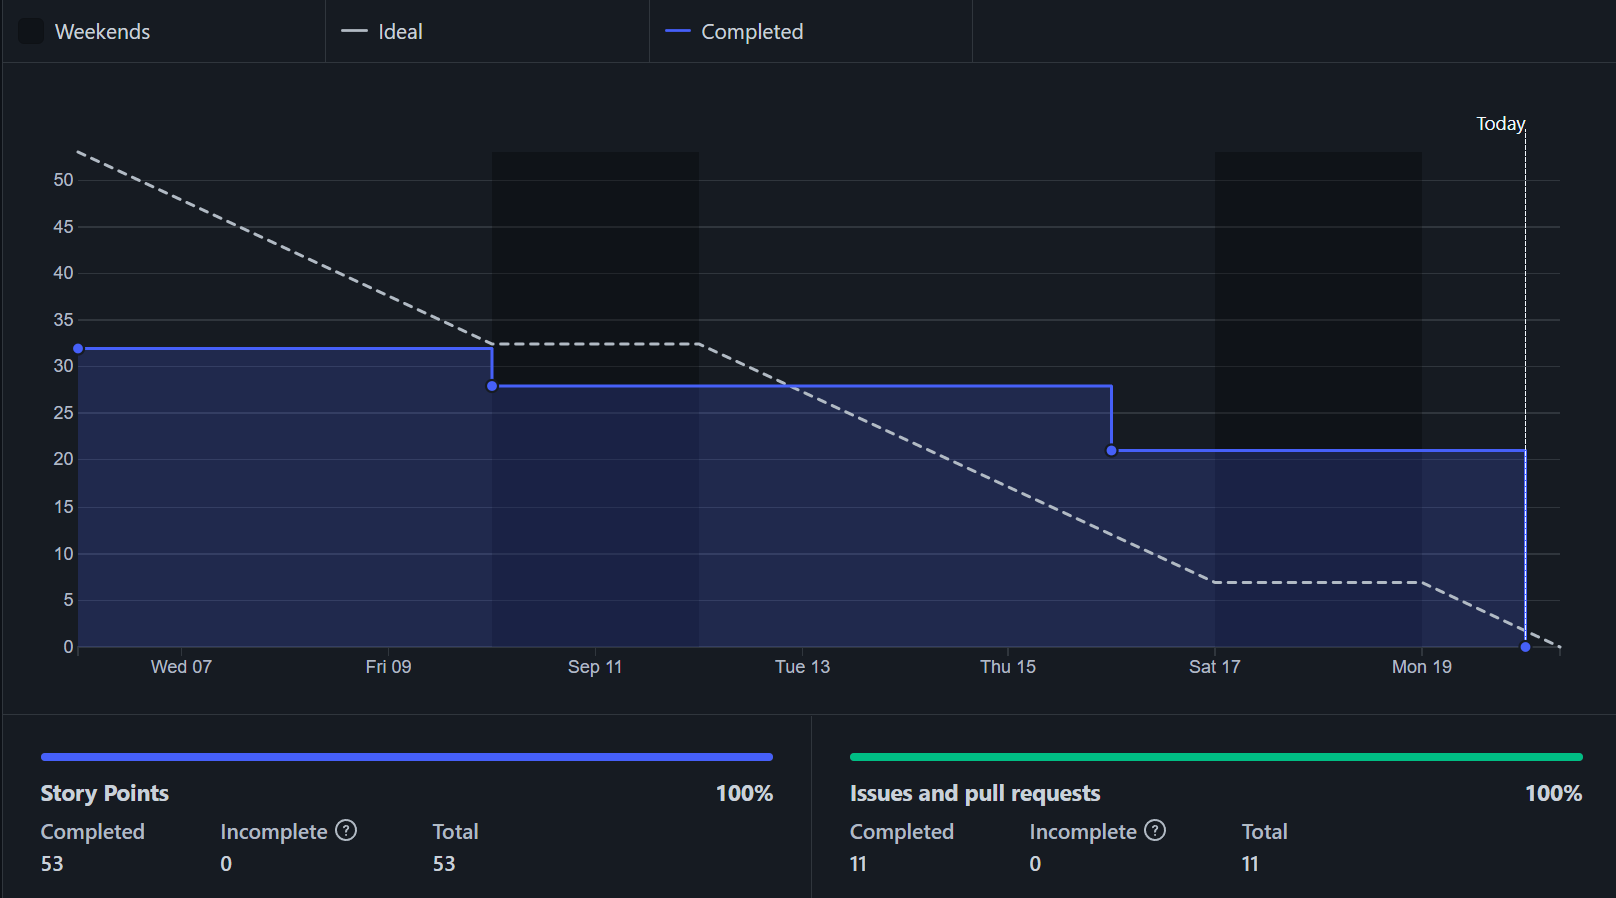
\includegraphics[width=0.8\textwidth]{img/sprint_06_20_sep.PNG}
\caption{Sprint: 06 Septiembre - 20 Septiembre, 2022}
\label{fig:sprint_06_20_sep}
\end{figure}

\section{Estudio de viabilidad}

En esta sección vamos a realizar un estudio de la viabilidad del proyecto tanto en el ámbito económico dando una aproximación de cuál sería la cantidad a pagar por un empresario, como de la viabilidad legal.

\subsection{Viabilidad económica}

De cara a la viabilidad económica vamos a centrarnos únicamente en el gasto que ha significado este proyecto, y no en el posible beneficio que podría dar. Para ello dividiremos los costes en cuatro:

\begin{itemize}
    \item Costes análisis
    \item Costes desarrollo
    \item Costes software
    \item Costes Hardware
\end{itemize}

\subsubsection{Costes análisis}

En cuanto a los costes de análisis en este proyecto solo ha trabajado un único analista web, que según Indeed \cite{indeed:oficial} el sueldo medio de un analista programador en España es de 28 350 € al año. Lo que estimaría una tarifa media de \textbf{19,68 €} por hora (28 350 / (30 horas x 48 semanas). Se han dedicado 10 semanas (estas semanas han sido en su mayoría antes de empezar el desarrollo, pero se han requerido algunos periodos temporales de análisis durante el desarrollo, ya cuantificados en esas 10 semanas)  al análisis del proyecto con jornadas de 6 horas diarias, es decir, unas 30 horas semanales.

30 horas/semana x 10 semanas x 19,68€/hora = \textbf{5 904 €} total

A este salario habría que añadirle los impuestos por seguridad social que actualmente aplicarían:

\begin{itemize}
    \item 23.6\% \textbf{contingencias comunes}.
    \item 5.5\% \textbf{tipo general de desempleo para contrato indefinido}.
    \item 0.20\% \textbf{FOGASA} (Fondo de Garantía Salarial).
    \item 0.60\% para \textbf{formación profesional}.
\end{itemize}

Estos datos (figuras \ref{fig:segsocial_contin} y \ref{fig:segsocial_otros}) provienen de la página de la Seguridad Social \cite{seguridad:social}, en el apartado de \textit{Régimen General de la Seguridad Social}.

\begin{figure}[h!] 
\centering
    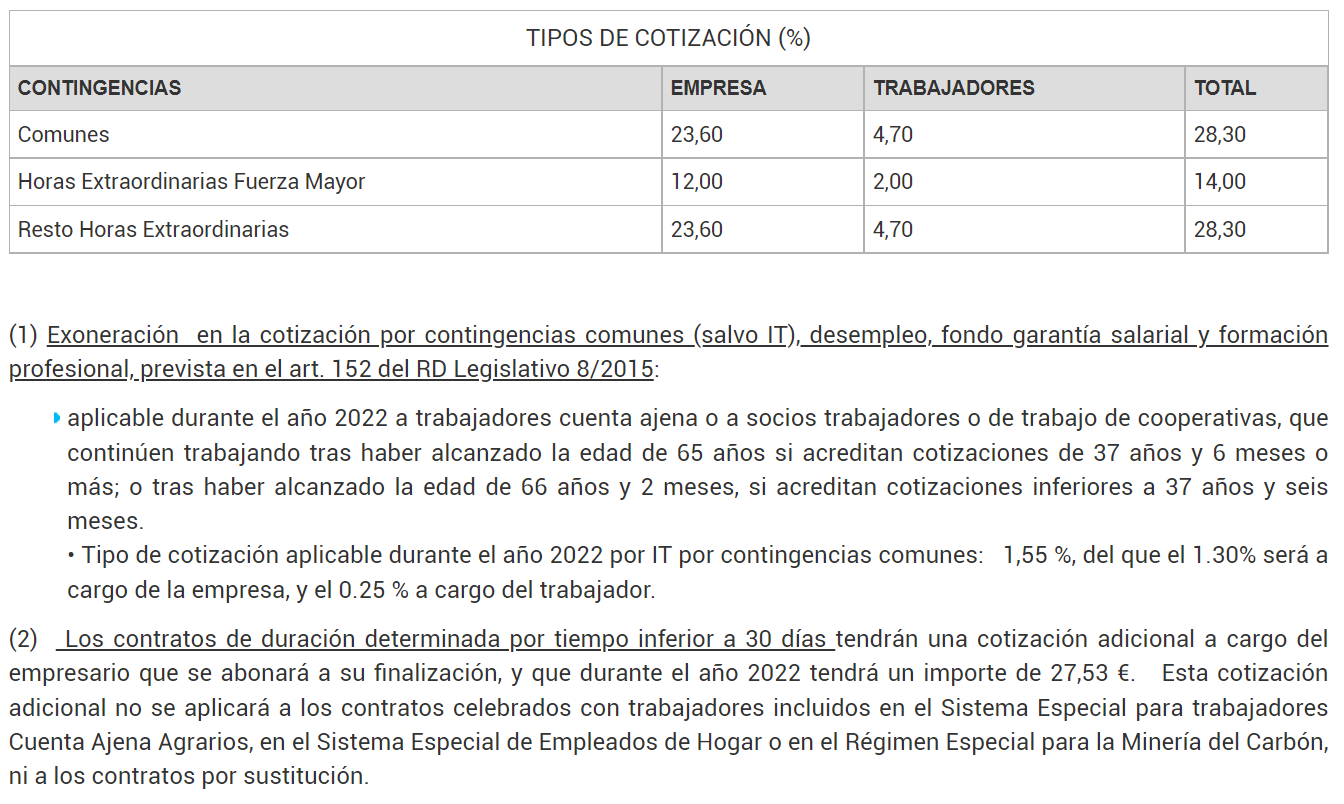
\includegraphics[width=0.8\textwidth]{img/seguridadsocial_1.PNG}
\caption{Régimen General de la Seguridad Social - Impuestos por contingencias comunes}
\label{fig:segsocial_contin}
\end{figure}

\begin{figure}[h!] 
\centering
    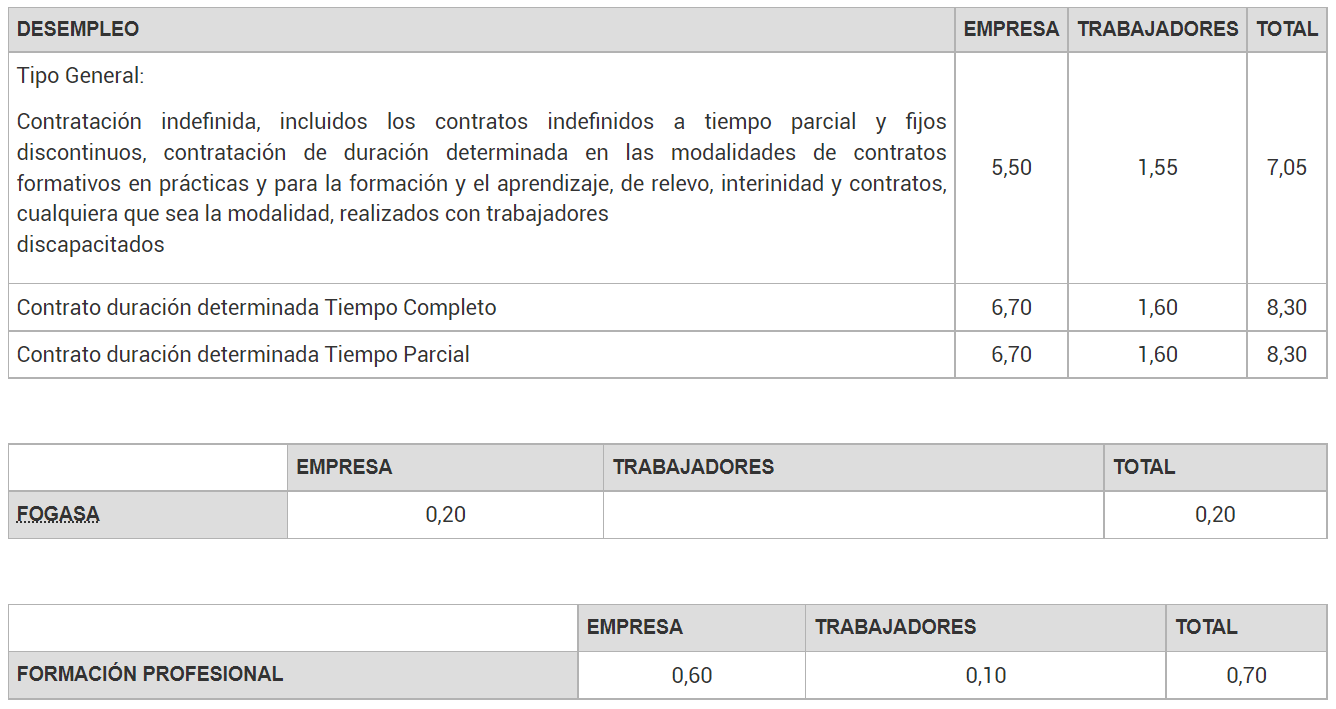
\includegraphics[width=0.8\textwidth]{img/seguridadsocial_2.PNG}
\caption{Régimen General de la Seguridad Social - Impuestos por otros}
\label{fig:segsocial_otros}
\end{figure}

El empleador debería añadir estos impuestos al total de pago tanto en la parte de desarrollo como de análisis.

$$ 5\:904 * (1 + 0,236 + 0,055 + 0,002 + 0,006) = \textbf{7 669, 296 €} $$


\subsubsection{Costes desarrollo}

En cuanto a los costes de desarrollo en este proyecto solo ha trabajado un único desarrollador web, que según Indeed \cite{indeed:oficial} el sueldo medio de desarrollador web en España es de 25 822 € al año. Lo que estimaría una tarifa media de \textbf{17,93 €} por hora (25 822 / (30 horas x 48 semanas). El proyecto se ha desarrollado en 5 periodos de 2 semanas con unas 6 horas al día, es decir, unas 30 horas semanales. 

30 horas/semana x (5 periodos x 2 semanas de duración) x 17,93€/hora = \textbf{5 379 €} (total trabajador sin impuestos)

Al igual que en el apartado anterior aplicamos los impuestos por seguridad social:

$$ 5\:379 \cdot (1 + 0,236 + 0,055 + 0,002 + 0,006) = \textbf{6 987,321 €} $$


\subsubsection{Costes software}

Las herramientas utilizadas son totalmente gratuitas. Por lo que no hay coste en este apartado. 

\subsubsection{Costes hardware}

El proyecto se ha desarrollado en un portátil Huawei KLVL-WXX9 con AMD Ryzen 7 4800h y 16GB de RAM con un precio de 700€ en enero de 2022. Partiendo que Hacienda marca que la amortización de ordenadores es de un 26\% multiplicado por 0,75 ( 11 meses de uso de noviembre 2021 a septiembre 2022, menos 2 meses de no trabajo da 9 meses de trabajo entre 12 que tiene el año da 0,75 siendo los meses de uso del portátil en un año) el portátil amortizado significaría una cantidad de 700 x 26\% = 182 al año, multiplicado por 0,75 = \textbf{136,5} seria el gasto en la duración de este proyecto.

Los gastos totales por tanto de este proyecto vienen representados en tabla de costes de la figura \ref{fig:costes_totales}.

\begin{table}[h]
    \centering
    \begin{tabular}{l c}
         \textbf{Tipo de Costes} & \textbf{Total } \\ 
         \hline
         \textit{Análisis} & 7 669, 296 € \\ 
         \textit{Desarrollo} & 6 987,321 € \\  
         \textit{Software} & 0 € \\ 
         \textit{Hardware} & 136,5 €   \\ 
         \hline
         \textbf{Total} & \textbf{14 793,117 €}\\ 
    \end{tabular}
    \caption{Tabla costes totales}
    \label{fig:costes_totales}
\end{table}


\subsection{Viabilidad legal}

Las herramientas utilizadas en el desarrollo del proyectos disponen de licencias gratuitas o son open source. En la tabla \ref{fig:herramientaslicense}  se muestra las licencias de cada herramientas utilizada.

\newpage

\begin{table}[h]
    \rowcolors{1}{}{lightgray}
    \centering
    \begin{tabular}{l c}
        \textbf{Herramientas} & \textbf{Licencia } \\ 
        \hline
        GitHub & GNU\\
        Visual Studio Code & MIT \\
        Debian & DFSG\\
        Angular & MIT\\
        Angular Translate & MIT\\
        Angular Material & MIT\\
        Bootstrap & MIT\\
        Node.js & MIT\\
        npm & MIT\\
        Heroku & EULA\\
        Netlify & MIT\\
        GLPK &  GPL\\
        \TeX{}Studio & GPL v2 \\
    \end{tabular}
    \caption{Licencias de herramientas utilizadas}
    \label{fig:herramientaslicense}
\end{table}

Uno de los requisitos del proyecto es que debe cederse bajo licencia GNU GPL 3.0. La GNU General Public License \cite{gnu:license} es una licencia libre y sin copyleft para software. Al contrario de la mayoría de licencias que se centran en restringir la libertad para compartir la obra, la licencia GNU esta destinada a garantizar su libertad al compartir y cambiar las versiones del programa. Siendo un proyecto de software libre.

La licencia GNU no impide la venta de las copias, cuando se habla de libertad se refiere a libertad de distribución de copias de software, pero no impide el cobrar por esas copias en caso de que el autor lo requiera.







